\section{Sparse matrix multiplication} \label{sec:spmm}
Sparse matrix multiplication leads to many random memory
accesses and its performance is usually limited by random memory throughput
of DRAM. We perform sparse matrix multiplication in semi-external memory (SEM)
to scale to a sparse matrix with billions of rows and columns. This strategy enables
nearly in-memory performance while achieving scalability in proportion
to the ratio of non-zero entries to rows or columns in a sparse matrix.

\subsection{Semi-external memory}
Our definition of semi-external memory for sparse matrix multiplication
keeps the sparse matrix on SSDs and the input dense matrix or some columns
of the input dense matrix in memory. During the computation, we stream
data in the sparse matrix from SSDs to maximize I/O throughput.

There are two options for keeping the output dense matrix. In applications
such as PageRank and many other graph
algorithms, dense matrices have only a few columns, so we can keep the output
dense matrix in memory. If a machine has insufficient
memory to keep the output matrix, we stream the output matrix
to SSDs or to the subsequent computation to reduce memory consumption and
potentially I/O as well.

In some applications such as non-negative matrix factorization (Section
\ref{sec:apps}), even the input dense matrix cannot fit in memory. In this case,
we partition the input dense matrix vertically so that each partition has
complete columns of the original input dense matrix and can fit in memory.
Each vertical partition stores elements in the row-major order to increase
data locality. For each partition, we perform sparse matrix multiplication
in semi-external memory as before and stream the output matrix to SSDs.
%This approach requires $\lceil \frac{D}{M} \rceil$ passes over the sparse
%matrix, where $D$ is the storage size of the input dense matrix and $M$ is
%the memory size.

\subsection{Sparse matrix format}
To support efficient sparse matrix multiplication on graphs in semi-external
memory, we need to use an alternative format for sparse matrices to increase
CPU cache hits and reduce I/O from SSDs. Compressed row
storage (CSR) or compressed column storage (CSC) format are not designed for
graphs and incur many CPU cache misses. They also require
a relatively large storage size. For a sparse matrix with billions of non-zero
entries, we have to use eight bytes to store row and column indices.

\begin{figure}
\centering
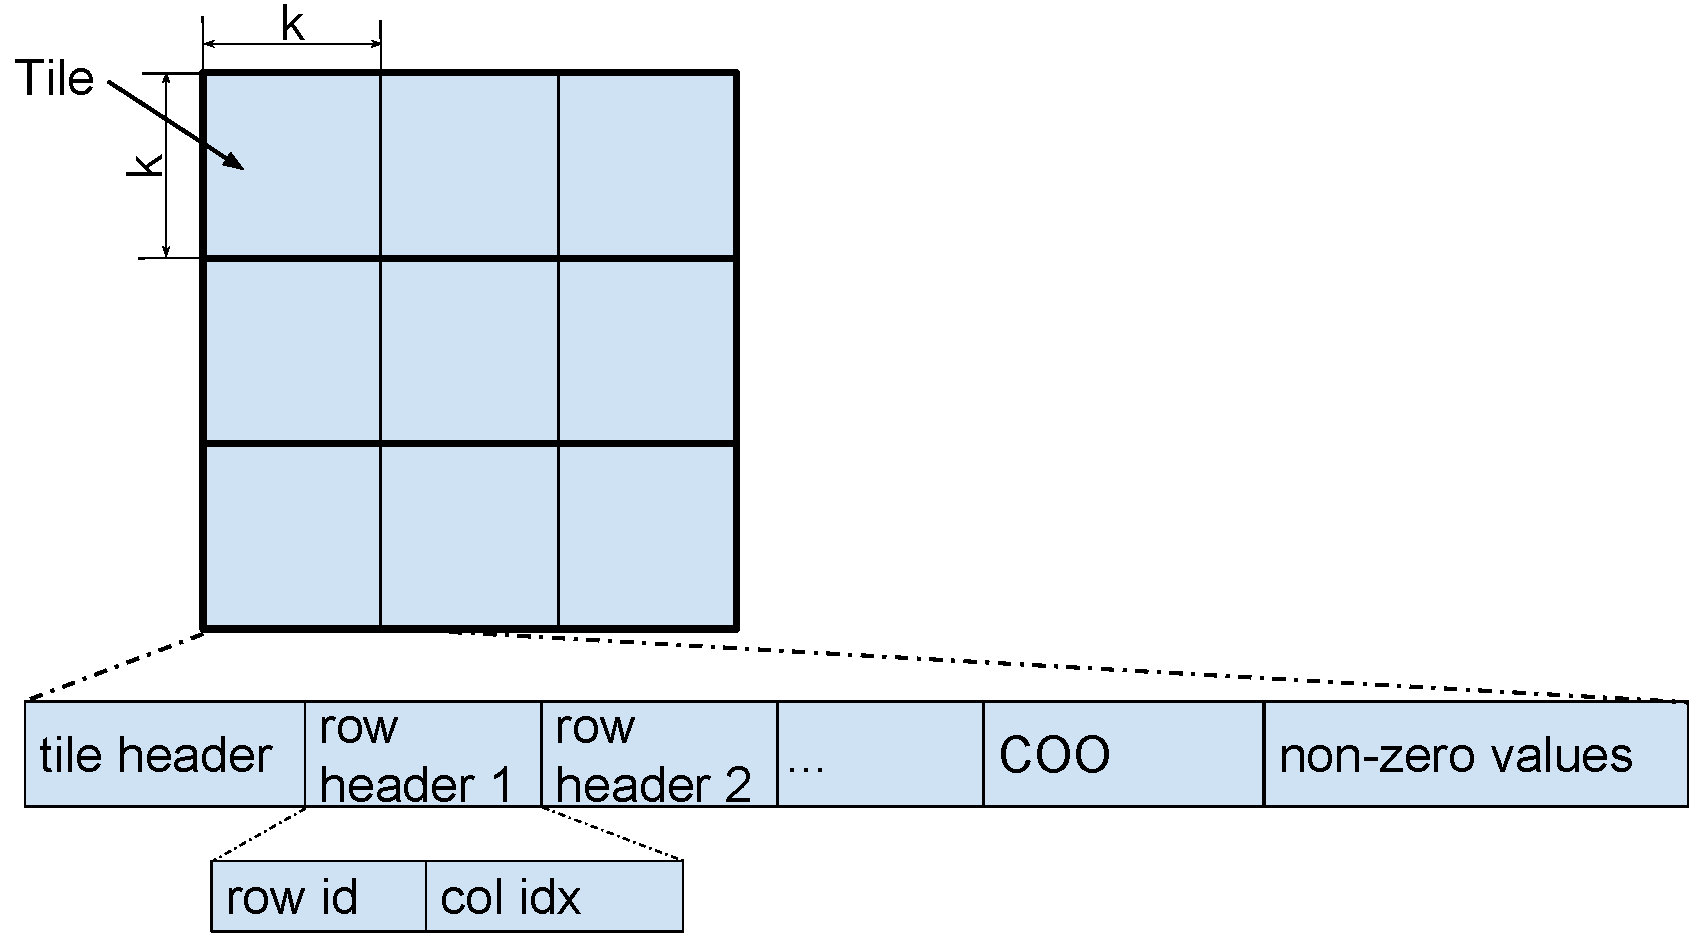
\includegraphics[scale=0.3]{SpMM_figs/sparse_mat.pdf}
\caption{The format of a sparse matrix.}
\label{sparse_mat}
\end{figure}

To increase CPU cache hits, we deploy cache blocking \cite{Im04} and store
non-zero entries of a sparse matrix in tiles (Figure \ref{sparse_mat}).
When a tile is small, the rows from the input and output dense matrices
involved in multiplication with the tile are always kept in the CPU cache
during the computation. The optimal tile size should fill the CPU cache
with the rows from the dense matrices and is affected by the number of columns
of the dense matrices. To handle dense matrices with different numbers
of columns, we deploy both static cache blocking and dynamic cache blocking.
We generate sparse matrices with a relatively small tile size and
rely on the runtime system
to optimize for different numbers of columns (Section \ref{sec:exec}).
However, a small tile size potentially increases the storage size of a sparse
matrix. In semi-external memory, the dense matrices usually have
a very small number of columns in sparse matrix multiplication. Therefore, we
use the tile size of $16K \times 16K$ by default to balance the matrix storage
size and the adaptibility to different numbers of columns.

\begin{figure}
\centering
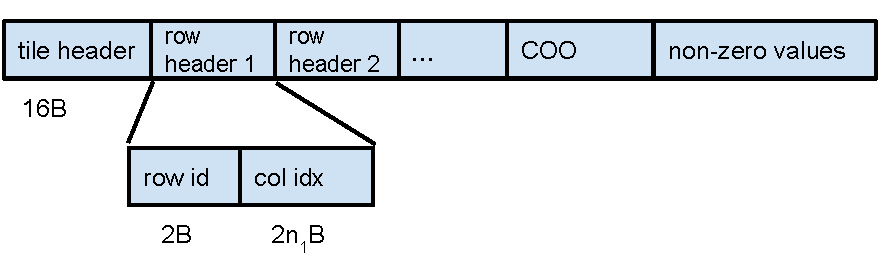
\includegraphics[scale=0.5]{SpMM_figs/tile_format.pdf}
\caption{The storage format (SCSR + COO) of a tile in a sparse matrix.}
\label{tile_format}
\end{figure}

We need a very compact format to store non-zero entries in a tile to reduce
the number of bits in a sparse matrix read from SSDs. A compact format is
performance critical because in semi-external memory SpMM SSDs
may be the bottleneck. In very sparse matrices many rows in a tile
do not have any non-zero entries. The CSR or CSC format wastes space because
they require an entry for each row/column in the row/column index. Doubly
compressed sparse column (DCSC) \cite{Buluc08} is proposed to avoid this problem
and is compact for hypersparse matrices such as submatrices of
a sparse matrix. However, even DCSC wastes space because it requires to store
pointers to columns and \dz{fails to reference to non-zero values with small
integers (e.g., two-byte integers)}.

We use a very compact format to store non-zero entries and refer to this
format as SCSR (Super Compressed Row Storage) (Figure \ref{tile_format}).
This format keeps data only for rows with non-zero entries in a tile and
maintains a row header for each non-empty row. A row header has an identifier
to indicate the row number, followed by column indices. 
The most significant bit of the identifier is always set to 1, while the most
significant bit of a column index entry is always set to 0. As such, we can easily
distinguish a row identifier from a column index entry and determine the end
of a row. Owing to the small size of a tile, we use two bytes to store a row
number and a column index entry, which further reduces the storage size. As such,
each non-zero entry requires at most four bytes to indicate its location in
a matrix. Because the most significant bit is used to indicate the beginning
of a row, this format allows a maximum tile size of $32K \times 32K$.

SCSR is
even more compact than DCSC \cite{Buluc08}. In the best case (each non-zero
entry is stored in a separate row/column), SCSR requires only 40\% of the space
than DCSC for binary sparse matrices. In the worst case (all non-zero entries
are stored in a single row/column), SCSR uses the same space as DCSC. Figure
\ref{fig:storage} shows that SCSR uses 45\%-70\% of the storage size used by
DCSC for large real-world graphs (Table \ref{graphs}). SCSR saves more space
in a sparse matrix where non-zero entries are more randomly distributed.

\begin{figure}
	\begin{center}
		\footnotesize
		\begin{tikzpicture}[gnuplot]
%% generated with GNUPLOT 4.6p4 (Lua 5.1; terminal rev. 99, script rev. 100)
%% Thu 26 May 2016 10:33:39 PM EDT
\path (0.000,0.000) rectangle (8.382,3.556);
\gpcolor{color=gp lt color border}
\gpsetlinetype{gp lt border}
\gpsetlinewidth{1.00}
\draw[gp path] (1.504,0.627)--(1.684,0.627);
\draw[gp path] (7.829,0.627)--(7.649,0.627);
\node[gp node right] at (1.320,0.627) { 0};
\draw[gp path] (1.504,1.139)--(1.684,1.139);
\draw[gp path] (7.829,1.139)--(7.649,1.139);
\node[gp node right] at (1.320,1.139) { 0.2};
\draw[gp path] (1.504,1.651)--(1.684,1.651);
\draw[gp path] (7.829,1.651)--(7.649,1.651);
\node[gp node right] at (1.320,1.651) { 0.4};
\draw[gp path] (1.504,2.162)--(1.684,2.162);
\draw[gp path] (7.829,2.162)--(7.649,2.162);
\node[gp node right] at (1.320,2.162) { 0.6};
\draw[gp path] (1.504,2.674)--(1.684,2.674);
\draw[gp path] (7.829,2.674)--(7.649,2.674);
\node[gp node right] at (1.320,2.674) { 0.8};
\draw[gp path] (1.504,3.186)--(1.684,3.186);
\draw[gp path] (7.829,3.186)--(7.649,3.186);
\node[gp node right] at (1.320,3.186) { 1};
\draw[gp path] (3.612,0.627)--(3.612,0.807);
\draw[gp path] (3.612,3.186)--(3.612,3.006);
\node[gp node left,rotate=-10] at (3.612,0.443) {Twitter};
\draw[gp path] (5.721,0.627)--(5.721,0.807);
\draw[gp path] (5.721,3.186)--(5.721,3.006);
\node[gp node left,rotate=-10] at (5.721,0.443) {Friendster};
\draw[gp path] (1.504,3.186)--(1.504,0.627)--(7.829,0.627)--(7.829,3.186)--cycle;
\node[gp node center,rotate=-270] at (0.246,1.906) {SCSR/DCSC};
\def\gpfillpath{(3.612,0.627)--(4.316,0.627)--(4.316,2.343)--(3.612,2.343)--cycle}
\gpfill{color=gpbgfillcolor} \gpfillpath;
\gpfill{color=gp lt color 0,gp pattern 0,pattern color=.} \gpfillpath;
\gpcolor{color=gp lt color 0}
\gpsetlinetype{gp lt plot 0}
\draw[gp path] (3.612,0.627)--(3.612,2.342)--(4.315,2.342)--(4.315,0.627)--cycle;
\def\gpfillpath{(5.721,0.627)--(6.424,0.627)--(6.424,2.419)--(5.721,2.419)--cycle}
\gpfill{color=gpbgfillcolor} \gpfillpath;
\gpfill{color=gp lt color 0,gp pattern 0,pattern color=.} \gpfillpath;
\draw[gp path] (5.721,0.627)--(5.721,2.418)--(6.423,2.418)--(6.423,0.627)--cycle;
\gpcolor{color=gp lt color border}
\gpsetlinetype{gp lt border}
\draw[gp path] (1.504,3.186)--(1.504,0.627)--(7.829,0.627)--(7.829,3.186)--cycle;
%% coordinates of the plot area
\gpdefrectangularnode{gp plot 1}{\pgfpoint{1.504cm}{0.627cm}}{\pgfpoint{7.829cm}{3.186cm}}
\end{tikzpicture}
%% gnuplot variables

		\caption{The ratio of the storage size required by SCSR and DCSC
			\cite{Buluc08} format for real-world graphs. SCSR is much more
		compact than DCSC for graphs.}
		\label{fig:storage}
	\end{center}
\end{figure}

Inside each cache tile of the SCSR, we use the coordinate format (COO) for
the rows that have only a single non-zero entry. For the adjacency matrices of
real-world graphs, many rows in a cache tile have only one non-zero entry,
owing to the sparsity of the graphs and nearly random vertex connection.
Iterating over single-entry rows in the SCSR format requires to test
the end of a row for every non-zero entry, which leads to many conditional jumps.
In contrast, COO is more suitable for storing these
single-entry rows. It does not increase the storage size but significantly
reduces the number of conditional jump instructions. As a result, we combine
SCSR with COO and store non-zero entries in the COO format behind the row headers
of SCSR (Figure \ref{tile_format}).

%We organize tiles in a sparse matrix in tile rows and maintain a matrix index
%for them. Each entry of the index stores the location of a tile row on SSDs
%to facilitate random access
%to tile rows. This is useful for parallelizing sparse matrix multiplication.
%Because a tile contains thousands of rows, the matrix index requires a very
%small storage size even for a billion-node graph. We keep the entire index
%in memory during sparse matrix multiplication.

\subsection{Dense matrices}
In many applications, the dense matrices in SpMM are
tall-and-skinny matrices with millions or even billions of rows but only a small
number of columns. The number of columns is determined by applications.
In semi-external memory,
we keep the input dense matrix in memory, so its size governs memory consumption
of sparse matrix multiplication. To increase data locality in SpMM, the elements
in the dense matrices are stored in row-major order.

For a non-uniform memory architecture (NUMA), we partition the input dense matrix
horizontally and store partitions evenly across NUMA nodes. The NUMA architecture
is prevalent in today's multi-processor servers, where each processor connects
to its own memory banks. Therefore, keeping partitions evenly across all NUMA
nodes helps to fully utilize the bandwidth of memory and inter-processor links.
For horizontal partitioning, we assign multiple contiguous rows in a row
interval to a partition, which is assigned to a NUMA node. A row interval
in a partition always has $2^i$ rows for efficiently locating a row
with bit operations. The row interval size is multiple of the tile size of
a sparse matrix so that multiplication on a tile only needs to access rows
from a single row interval.

%\begin{figure}
%\centering
%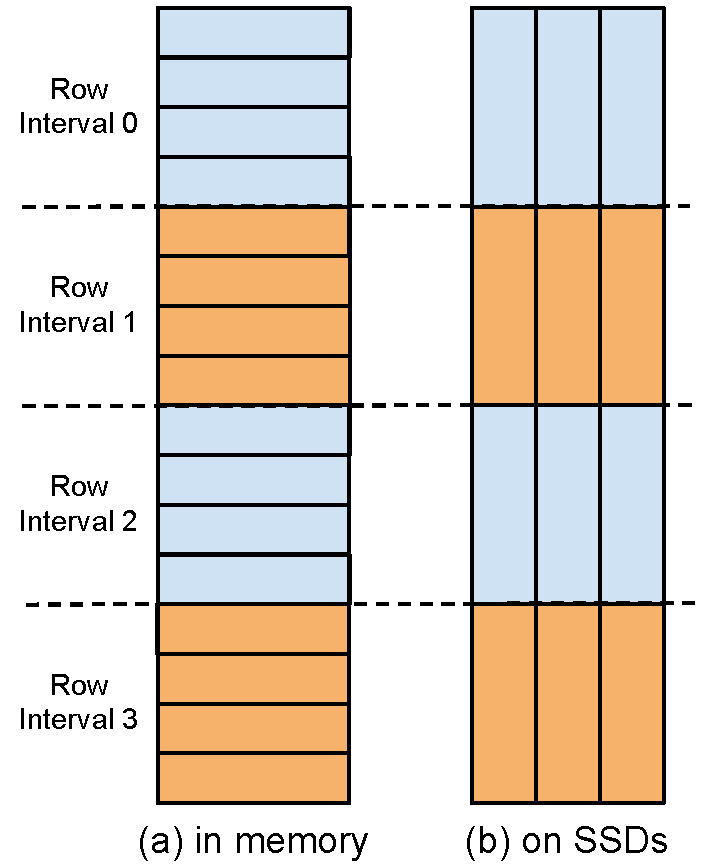
\includegraphics[scale=0.4]{./dense_matrix.pdf}
%\caption{The data layout of tall-and-skinny dense matrices. It is partitioned
%	horizontally into many row intervals.
%(a) In the input dense matrix of SpMM, row intervals are stored across NUMA nodes and
%elements are stored in the row-major order; (b) in the eigensolver, elements
%in a dense matrix inside a row interval are stored in the column-major order;
%(c) in NMF, a dense matrix is partitioned vertically first and in each partition,
%elements are stored in the row-major order.}
%\label{dense_mat}
%\end{figure}

\begin{algorithm}
	\caption{Perform sparse matrix multiplication on tile rows of a sparse
	matrix in a thread.}
	\label{alg:spmm}
	\begin{algorithmic}[1]
		\Procedure{ProcessTileRows}{trQueue}
		\While{$|trQueue| > 0$}
		\If {$|trQueue| > thres$} \State $numTRs \gets superTileSize$
		\Else \State $numTRs \gets 1$
		\EndIf
		\State $trs \gets get\_tile\_rows(trQueue, numTRs)$
		\State $read\_async(trs, callback=ProcessSTRow)$
		\If {$pendingIOs > maxIOs$} \State wait for I/O
		\EndIf
		\EndWhile
		\EndProcedure

		\State

		\Procedure{ProcessSTRow}{trs, inMat, outMat}
		\State $outBuf \gets matrix(0, nrow(tile), ncol(inMat))$
		\State $sts \gets get\_super\_tiles(trs)$
		\For{$st \in sts$}
		\State $tiles \gets get\_tiles(st)$
		\For{$tile \in tiles$}
		\State $lInMat \gets$ rows from $inMat$ for $tile$
		\State $lOutMat \gets$ rows from $outBuf$ for $tile$
		\State $lOutMat += tile * lInMat$
		\EndFor
		\EndFor
		\State $write\_async(outMat, outBuf)$
		\EndProcedure
	\end{algorithmic}
\end{algorithm}

\subsection{Parallel Execution} \label{sec:exec}
When parallelizing sparse matrix multiplication, we take into account
semi-external memory and the power-law distribution of non-zero entries
in each row of a sparse matrix.

Semi-external memory favors horizontal partitioning on a sparse matrix
for parallelization because this partitioning
scheme minimizes writes to SSDs and remote memory with small memory
consumption. Horizontal partitioning requires only the thread assigned tile
rows to allocate local memory buffers for intermediate results when the thread
goes through all tiles in the tile rows. All intermediate computation
results on tiles are merged into the local memory buffers, which results in
writing the output matrix at most once to SSDs and no remote memory writes.
This is essential for semi-external memory computation because
saved memory can be used to keep more columns in the input dense matrix in
memory to reduce I/O from SSDs (as discussed in Section \ref{sec:mem}).
In contrast, both vertical partitioning and 2D partitioning requires each
thread to maintain a local memory buffer for the same tile rows in order
to reduce writes to SSDs and remote memory.
%Horizontal partitioning also allows a small matrix index to
%locate non-zero entries in a sparse matrix quickly, because we only need to
%locate tile rows. As such, the matrix index is tiny even for a sparse matrix
%with billions of rows, permitting us to keep the entire matrix index in memory.

For parallel computation, each thread runs \textit{ProcessTileRows} (in Algorithm
\ref{alg:spmm}) that gets computation tasks (tile rows) from a global task queue
\textit{trQueue} to achieve load balancing and large I/O writes to SSDs.
%The global task queue is the only data structure that incurs
%concurrent writes from threads in our semi-external sparse matrix multiplication.
At the beginning, a thread gets larger computation tasks (several tile rows
at a time); as the computation approaches completion, a thread gets smaller
tasks (one tile row at a time). This design reduces concurrent access to
the global data structure while realizing good load balancing. When a thread
gets a computation task, it reads the corresponding tile rows asynchronously,
and invokes the callback function \textit{ProcessSTRow} to process the tile rows
once I/O is complete.
$get\_tile\_rows()$ controls a global execution order to ensure that all threads
are processing contiguous tile rows so that we can merge writes for computation
results.

When processing tile rows, we organize tiles into super tiles to better utilize
the CPU cache. The tile size of a sparse
matrix is specified when the sparse matrix image is created and is relatively
small to handle different numbers of columns in the dense matrices. A super tile
is composed of tiles from multiple contiguous tile rows (Figure \ref{sparse_mat})
and its size is determined at runtime by three factors: the number of columns
in the dense matrices, the CPU cache size and the number of threads that
share the CPU cache. An optimal size for a super tile fills
the CPU cache with the rows from the dense matrices involved in
the computation with the super tile.

\textit{ProcessSTRow} in Algorithm \ref{alg:spmm} processes tile rows.
It splits the input tile rows into super tiles with $get\_super\_tiles$ and
then further into tiles with $get\_tiles$. It processes all tiles in a super
tile before moving to the next one. As such, the computation on a tile reuses
data in the CPU cache from the computation on the previous tile. We maintain
a local memory buffer $outBuf$ to store the computation results,
which minimizes remote memory access. Once the computation in \textit{ProcessSTRow}
is complete, $outBuf$ contains complete results and is written back to
SSDs asynchronously with $write\_async()$. The computation result from a task
may be small. Instead of writing the result immediately, $write\_async()$ may
postpone the write and merge it with ones from other threads so that we can
write them to SSDs with a single I/O.

In spite of nearly random edge connection in a real-world graph, we explore
regularity in multiplying a tile with a partition of a row-major dense matrix.
In this case we multiply a non-zero entry from a tile with all elements in
a row of the input dense matrix and add the results to the corresponding row
of the output dense matrix.
We perform these operations with vector CPU instructions, such as
AVX \cite{avx} to enable more efficient memory access and computation.
The current implementation relies on GCC's auto-vectorization
to translate the C code to vector CPU instructions by predefining the matrix
width in the code.

\subsection{I/O optimizations}
Semi-external memory sparse matrix multiplication streams a sparse matrix from
SSDs, which results in sequential I/O. This I/O access pattern does not generate
any cache hits in the Linux page cache when the sparse matrix size is larger
than main memory. As such, we access a sparse matrix on SSDs with direct I/O.
For accessing data in fast SSDs sequentially, the overhead of operating systems
such as thread context switch and memory allocation becomes noticeable.
We tackle these obstacles to maximize I/O throughput.

We issue asynchronous I/O and poll for I/O to avoid thread
context switches because the latency of a context switch can undermine
the sequential I/O throughput of a high-speed SSD array. When a thread issues
an I/O request and waits for I/O completion, the operating system switches
the thread
out; the operating system reschedules the thread for execution once I/O is
complete. However, there is latency for thread rescheduling and the latency
from frequent rescheduling can cause noticeable performance degradation
on a high-speed SSD array. As such, we use I/O polling to avoid a thread from
being switched out after the thread completes all computation available to it.

When accessing a sparse matrix or a dense matrix from SSDs, we maintain a set of
memory buffers for I/O access to reduce the overhead of memory allocation.
We use large I/O to access matrices on SSDs to increase I/O throughput.
Large memory allocation is expensive because the operating
system usually allocates a large memory buffer with \textit{mmap()} and
populates the buffer with physical pages when it is used. Therefore, we keep
a set of memory buffers allocated previously and reuse them for new I/O requests.
For accessing a sparse matrix, tile rows usually have different sizes, so we resize
a previously allocated memory buffer if it is too small for a new I/O request.

\subsection{The impact of the memory size on I/O}
\label{sec:mem}
More memory reduces I/O in semi-external memory.
The minimum memory requirement for semi-external memory sparse matrix
multiplication is $n c + t \epsilon$, where $n$ is the number of rows
of the input dense matrix, $c$ is the element size in bytes,
$t$ is the number of threads processing the sparse matrix
and $\epsilon$ is the buffer size for the sparse matrix and the output
dense matrix. When a machine does not have sufficient memory to keep the entire
input dense matrix in memory, we need multiple passes on the sparse matrix to
complete the computation. Reducing memory consumption is essential
to achieve performance in semi-external memory. By keeping more columns of
the input dense matrix in memory, we reduce the number of I/O passes.

When a machine does not have sufficient memory to keep the entire input dense
matrix, we use the existing memory to keep as many columns in the input
dense matrix in memory as possible. Although we can use some memory to cache
part of the sparse matrix,
keeping more columns of the input dense matrix in memory saves more I/O than
using the same amount of memory to cache the sparse matrix. Assume the input
dense matrix has $n$ rows and $k$ columns. Again, $c$ is the element size
in bytes. The storage size of the sparse
matrix is $E$ bytes and the memory size is $M$ bytes. We further assume
we use $M'$ bytes to keep some columns of the dense matrices in memory
($M' < M$, ${n c k} \mod {M'} \equiv 0$)
and the remaining memory ($M - M'$) to cache the sparse matrix.
The amount of data in the sparse matrix read from SSDs is
\begin{equation*}
IO_{in} = \frac{n c k}{M'} [E - (M - M')]
\end{equation*}
Because $E > M$ in semi-external memory, we minimize $IO_{in}$ by maximizing $M'$.
Therefore, using memory for the input dense matrix always results in a smaller
amount of I/O than using memory for caching the sparse matrix.

As the number of columns in memory from the input dense matrix increases,
the bottleneck of the system
may switch. When we keep only one column of the input dense matrix in memory,
the system is usually I/O bound; when we keep more columns of the dense matrix
in memory, the system will become CPU bound and the I/O complexity does not
affect its performance.
%and the additional memory does not improve
%the performance of sparse matrix multiplication further.

%Our strategy results in the minimum amount of data written to SSDs. When the output
%dense matrix cannot fit in memory, the maximum write is $N k$ for a square
%sparse matrix.
%In other words, the output matrix only needs to be written to SSDs at most once.
%The additional memory in the system can be used to buffer part of the output
%dense matrix to reduce the amount of data written to SSDs. Streaming the output
%matrix directly to the subsequent matrix computation can also reduce data written
%to SSDs.

\subsection{I/O complexity}
The semi-external memory (SEM) solution for sparse matrix multiplication leads
to no more I/O than the external-memory (EM) solution for many real-world graphs.

When a machine has sufficient memory to keep the entire input dense matrix
in memory, the SEM solution only needs to read the sparse matrix and the input
dense matrix once and write the output dense matrix once. This is
the minimum amount of I/O.

When a machine has insufficient memory to keep the input dense matrix, the SEM
solution still leads to less I/O than the EM solution when $E < n c k t$ if we
minimize writes to SSDs.
In this analysis, we assume a square sparse matrix. The same analysis applies
to a rectangular sparse matrix as well.
In this case, the SEM solution scans the sparse matrix multiple times.
\begin{equation*}
read_{SEM} = \frac{n c k}{M} E + n c k
\end{equation*}
To minimize writes, the EM solution
scans the sparse matrix once but reads the input dense matrix multiple times.
Due to near random vertex connection in real-world graphs, the EM solution needs to
read the entire input dense matrix each time. In the parallel setting,
the EM solution requires each thread to keep local memory buffers for portions
of the input and output dense matrices. Assume the EM solution keeps $j$ rows
from the input dense matrix and $i$ rows from the output dense matrix in memory
in each thread.
\begin{equation*}
(i c k + j c k) t = M \implies i < \frac{M}{c k t}
\end{equation*}
\begin{equation*}
read_{EM} = \frac{n}{i} n c k + E \implies  read_{EM} > \frac{n^2 c^2 k^2 t}{M} + E
\end{equation*}
When $n c k < E < n c k t$, $read_{EM} > read_{SEM}$.
When $E \leq n c k$, $read_{EM} > read_{SEM}$ for any $t \geq 2$.

As such, the SEM solution in practice causes less I/O in many natural graphs.
For the natural graphs that we have seen, such as Twitter \cite{twitter},
the Page graph \cite{web_graph} and Friendster \cite{friendster}, the number
of edges is of $10-100 \times$ the number of vertices. Essentially,
natural graphs have sparse edge matrices. We target multi-core machines with
10s to 100s of threads. For most of our applications, $k$ is of size 1-30.
For very small $k$, the SEM solution can keep the entire input dense matrix
in memory and leads to the minimum I/O. For a relatively larger $k$, $E < n c k t$
holds for most of natural graphs when the graphs are processed in a large
parallel machine. Therefore, the SEM solution usually performs less I/O than EM.

\section{Applications} \label{sec:apps}
We apply sparse matrix multiplication to three important applications widely
used in data mining and machine learning: PageRank \cite{pagerank},
eigensolver \cite{anasazi} and non-negative matrix factorization \cite{nmf}.
Each application demonstrates a different strategy of using memory for sparse
matrix multiplication.

\subsection{PageRank} \label{sec:pagerank}
PageRank is an algorithm to rank the Web pages by using hyperlinks between Web
pages. It was first used by Google and is identified as one of the top 10 data
mining algorithms \cite{top10}. PageRank is a representative of a set of graph
algorithms that can be expressed with sparse matrix multiplication or generalized
sparse matrix multiplication. Other important examples are label propagation
\cite{label_prop} and belief propagation \cite{Yedidia03}. The algorithm runs
iteratively and its update rule for each Web pages in an iteration is
\begin{equation*}
PR(u) = \frac{1-d}{N} + d \sum\limits_{v \in B(u)} \frac{PR(v)}{L(v)}
\end{equation*}
where $B(u)$ denotes the neighbor list of vertex $u$ and $L(v)$ denotes
the out-degree of vertex $v$. %We implement the PageRank algorithm with sparse
%matrix multiplication (Figure \ref{code:pagerank}).


%\begin{figure}
%\centering
%%\begin{minted}[mathescape, fontsize=\scriptsize,]{r}
%\begin{lstlisting}
%while (L1 >= epsilon && niters < max.niters) {
%	pr2 <- d/N+(1-d)*(A %*% (pr1/out.deg))
%	L1 <- sum(abs(pr1-pr2))
%	pr1 <- pr2
%	niters <- niters + 1
%}
%\end{lstlisting}
%%\end{minted}
%\caption{The implementation of PageRank \cite{pagerank} with SpMM.}
%\label{code:pagerank}
%\end{figure}

%Based on the memory size, we can place different data in memory to reduce I/O.
%When the memory can only fit a single vector, each iteration needs
%to write a vector to SSDs and read two vectors (the result from
%the previous iteration and the degree vector) and the sparse matrix
%from SSDs. When the memory can fit two vectors, the output vector can be kept
%in memory, so each iteration needs to read the sparse matrix and the degree vector
%and does not write any data to SSDs. As more memory can be used, we can
%further keep the degree vector and even cache part of the sparse matrix.

\subsection{Eigensolver}
An eigensolver is another commonly used application that requires sparse matrix
multiplication. Many algorithms \cite{Lanczos, IRLM, krylovschur} and frameworks
\cite{arpack, anasazi, slepc} have been developed to solve a large eigenvalue
problem.

We take advantage of the Anasazi eigensolver framework \cite{anasazi} and
replace its original matrix operations with our SEM sparse
matrix multiplication and external-memory dense matrix operations. To compute
eigenvalues of a $n \times n$ matrix, many eigenvalue algorithms for a large
sparse matrix require to construct a vector subspace with a sequence of
sparse matrix multiplications and each vector in the subspace has the length of $n$.
Due to the sparsity of real-world graphs, the vector subspace is large and we keep
vectors in the subspace on SSDs. In addition to sparse matrix
multiplication, eigensolvers perform some dense matrix operations on the subspace.
For example, eigensolvers need to orthogonalize the vectors in the subspace with
dense matrix multiplication. The Anasazi eigensolvers have block extension to
update multiple vectors in the subspace simultaneously, which results in sparse matrix dense
matrix multiplication. The most efficient Anasazi eigensolver on sparse graphs
is the KrylovSchur eigensolver \cite{krylovschur}, which updates a small number
of vectors (1-4) in the subspace simultaneously. Zheng et al.
\cite{flasheigen} provides the details of extending the Anasazi eigensolver
with external-memory matrix operations.

%The choice of data placement for an eigensolver is a little different from
%PageRank. If a machine has a small amount of memory, the memory should be
%used to keep the input dense matrix. If a machine has more memory, we should
%use it to buffer the output dense matrix. The dense matrices involved in
%sparse matrix multiplication have a small number of columns in
%the KrylovSchur eigensolver and usually can fit in memory. 
%Additional memory should be used to buffer the vectors in the subspace
%to reduce I/O for dense matrix operations.

\subsection{Non-negative matrix factorization}
Non-negative matrix factorization (NMF) \cite{nmf} finds two non-negative
low-rank matrices $W$ and $H$ to approximate a matrix $A \approx WH$. NMF
has many applications in machine learning
and data mining. A well-known example is collaborative filtering \cite{cf} in
recommender systems. NMF can also be applied to graphs to find communities
\cite{yang13, wang11}.

Many algorithms are designed to solve NMF and here we describe an algorithm
\cite{nmf} that requires a sequence of sparse matrix multiplications.
The algorithm uses multiplicative update rules and updates matrices $W$ and $H$
alternately. In each iteration, the algorithm first fixes $W$ to update $H$
and then fixes $H$ to update $W$.
\begin{equation*}
H_{a\mu} \leftarrow H_{a\mu} \frac{{(W^TA)}_{a\mu}}{{(W^TWH)}_{a\mu}},
W_{ia} \leftarrow W_{ia} \frac{{(AH^T)}_{ia}}{{(WHH^T)}_{ia}}
\end{equation*}

We apply SEM sparse matrix multiplication to NMF differently
based on the memory size and the number of columns in $W$ and $H$. Due to
the sparsity of a graph, $W$ and $H$ may require storage as large as
the sparse matrix and can no longer fit in
memory. Therefore, we partition $W$ and $H$ vertically and run multiple
sparse matrix multiplications to compute $W^TA$ and $AH^T$, if the memory is not
large enough.

%The choices of data placement for NMF are
%shown as follows. If memory is small, all memory should be used to keep as many
%columns in the input dense matrix as possible to reduce I/O. The original sparse
%matrix multiplication is broken into multiple multiplications. We stream the output
%dense matrices to SSDs and construct some of the input dense matrices for the next
%sparse matrix multiplications in memory to reduce the latency of loading
%the input dense matrix to memory. The additional memory in a machine can be used
%to buffer the output dense matrix of sparse matrix multiplication.
